
\chapter{Soluzioni computazionali quantistiche}

Dopo aver esplorato il problema elettronico e le tecniche classiche, l’emergere dei computer quantistici apre nuove prospettive per affrontare i sistemi chimici più complessi. In questo capitolo, si introducono i concetti fondamentali della computazione quantistica, come \textbf{qubit}, \textbf{gates} e \textbf{circuiti}, gettando le basi per approcci innovativi come gli algoritmi variazionali quantistici.


% ==============================================================================================================
\section{Introduzione al quantum computing}

% --------------------------------------------------------------------------------------------------------------
\subsection{Qubit}

Un \textbf{qubit} è un qualsiasi sistema fisico a due livelli, generalmente indicati con $\ket{0}$ e $\ket{1}$, e rappresenta l'unità fondamentale di informazione del quantum computing. 
Mentre un \inglese{bit} classico può assumere soltanto due valori, 0 oppure 1, un \inglese{quantum bit} può esistere in una sovrapposizione qualsiasi dei due stati \cite{FernandezCombarro2020,Nielsen_Chuang_2010}:

\begin{equation}\label{eqn:qubit}
    \ket{q} = \alpha \ket{0} + \beta \ket{1}
\end{equation}

dove $\alpha,\beta\in\mathbb{C}$ sono le ampiezze di probabilità dei due stati e pertanto soddisfano la condizione:

\begin{equation}\label{eqn:misura-unitaria}
    |\alpha|^2 + |\beta|^2 = 1
\end{equation}

% ..............................................................................................................
\subsubsection{Sfera di Bloch}

Attraverso semplici manipolazioni algebriche, rispettando la condizione di unitarietà (eq. \ref{eqn:misura-unitaria}) e considerando che una fase globale non ha un effetto fisico visibile, è possibile riscrivere la \ref{eqn:qubit}:

\begin{equation}\label{eqn:bloch}
    \ket{q} = \cos \frac{\theta}{2} \ket{0} + e^{i\varphi} \sin \frac{\theta}{2} \ket{1}
\end{equation}

questa relazione offre una comoda rappresentazione, che permette di visualizzare il qubit in maniera intuitiva: le variabili $\theta$ e $\phi$ individuano un punto nello spazio posizionato sulla superficie di una sfera unitaria, detta \textbf{sfera di Bloch}.

\begin{figure}[H]
    \centering
    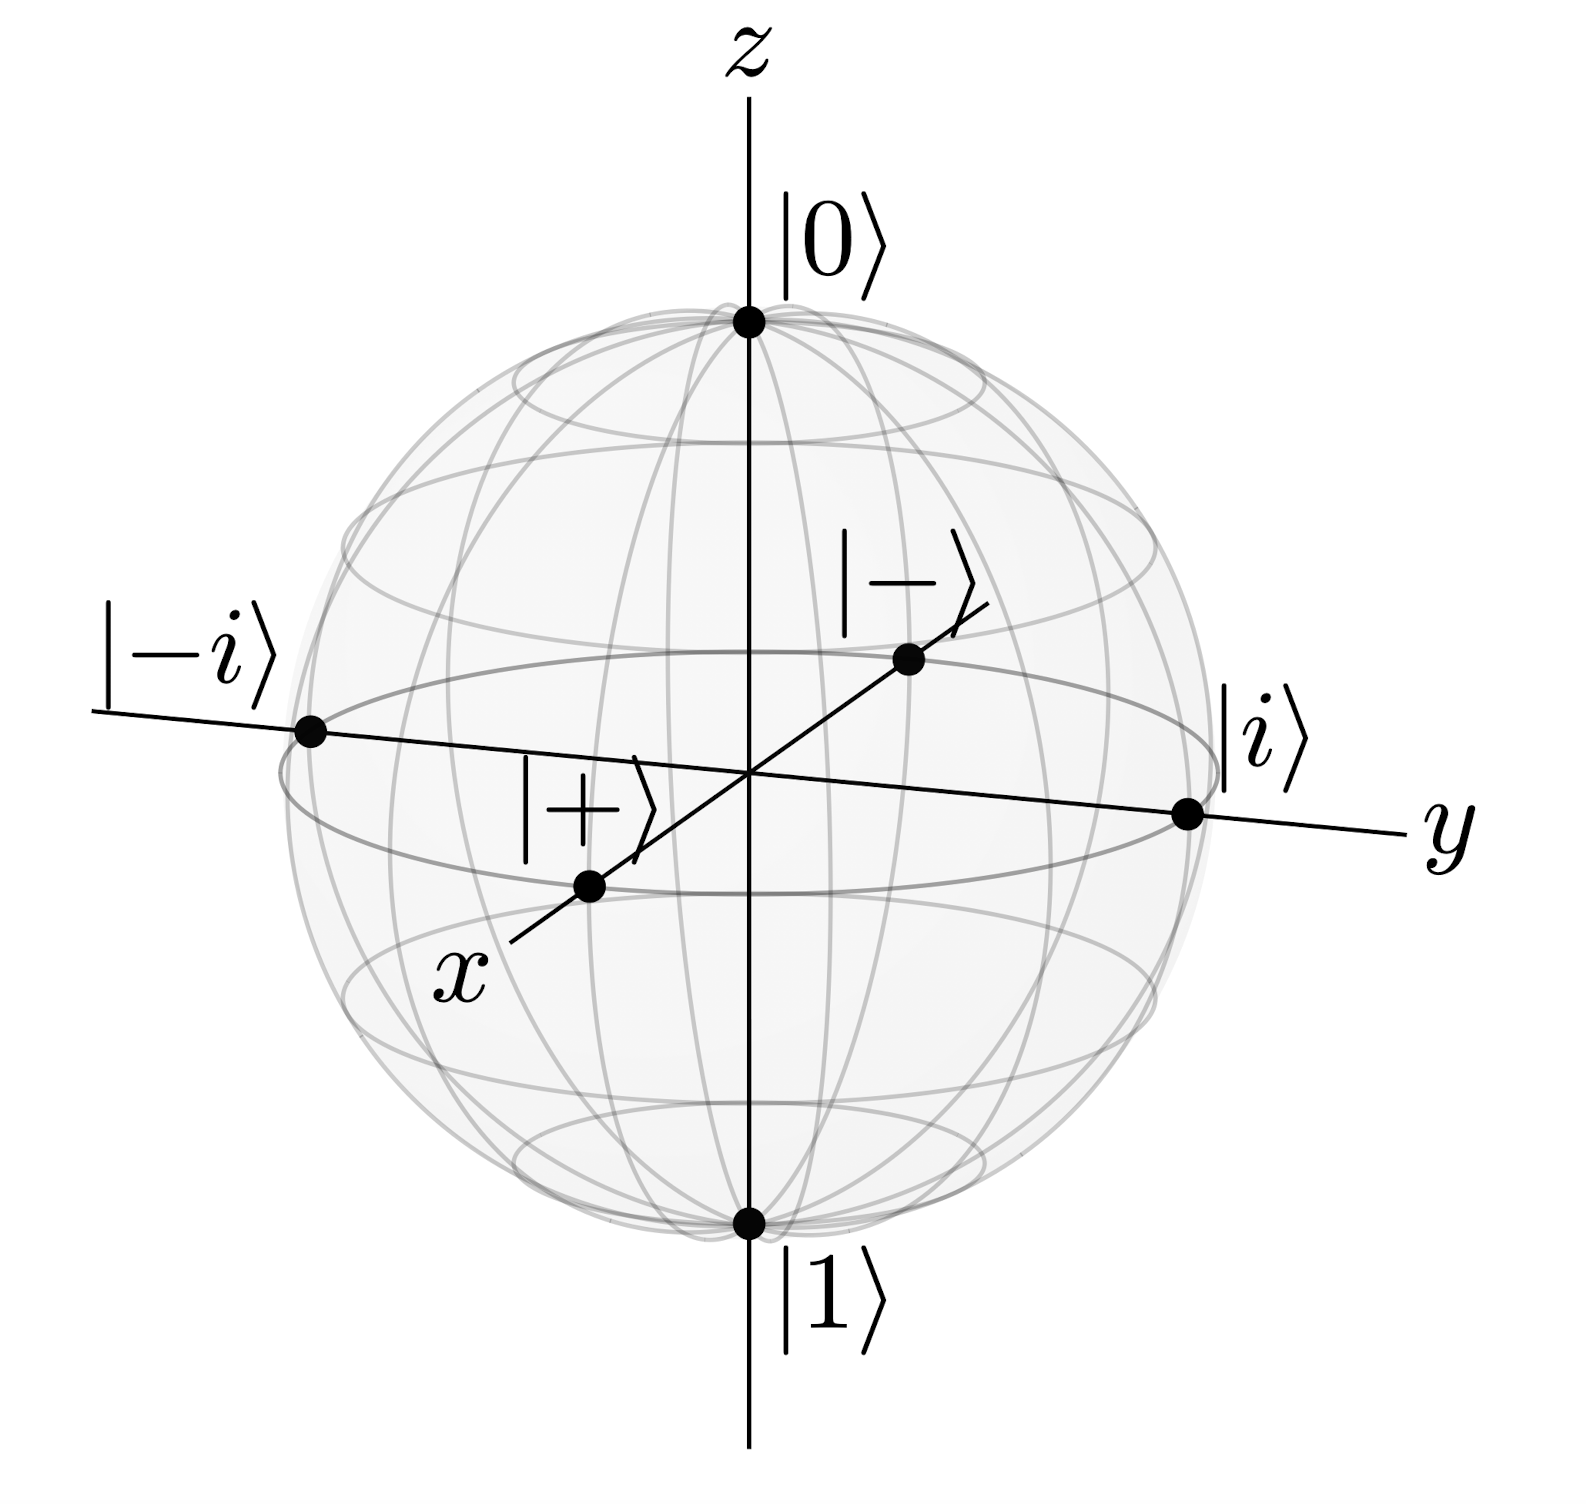
\includegraphics[width=0.5\textwidth]{Immagini/Capitolo_2/bloch.png}
    %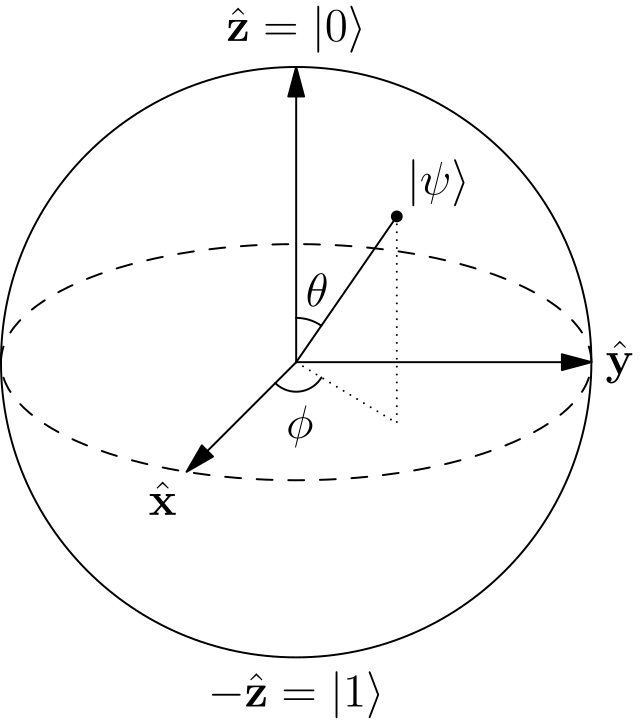
\includegraphics[width=0.5\textwidth]{Immagini/Capitolo_2/bloch.svg.png}
    \caption{Sfera di Bloch \cite{Wong2022}.}
    \label{fig:sfera-di-Bloch}
\end{figure} 

I punti ai poli della sfera sono identificati dagli stati $\ket{0}$, $\ket{1}$ che insieme formano la cosiddetta \textbf{base computazionale} $\{\ket{0},\ket{1}\}$. Allo stesso modo, i punti agli antipodi sugli assi $x$ e $y$ corrispondono ciascuno ad una base bidimensionale, spesso indicate con $\{\ket{+},\ket{-}\}$ e $\{\ket{+i},\ket{-i}\}$, i cui elementi possono essere sviluppati sulla base computazionale:

\begin{subequations}\label{eqn:autostati-rotazioni}
\small
\begin{align}
    &\ket{0} = \vectorTwo{1}{0} &&\ket{1} = \vectorTwo{0}{1}\\
    &\ket{+} = \frac{\ket{0}+\ket{1}}{\sqrt{2}} = \frac{1}{\sqrt{2}} \vectorTwo{1}{1} 
    &&\ket{-} = \frac{\ket{0}-\ket{1}}{\sqrt{2}} = \frac{1}{\sqrt{2}} \vectorTwo{1}{-1}\\
    &\ket{+i} = \frac{\ket{0}+i\ket{1}}{\sqrt{2}} = \frac{1}{\sqrt{2}} \vectorTwo{1}{i} 
    &&\ket{-i} = \frac{\ket{0}-i\ket{1}}{\sqrt{2}} = \frac{1}{\sqrt{2}} \vectorTwo{1}{-i}
\end{align}
\end{subequations}

% ..............................................................................................................
\subsubsection{Informazione di un qubit}

Per caratterizzare univocamente uno stato $\ket{q}$ occorrono due numeri reali indipendenti, che lo collocano in uno degli infiniti punti sulla sfera di Bloch; si potrebbe allora pensare che un qubit possa memorizzare una quantità di informazioni virtualmente illimitata. Tuttavia, per la natura quantistica del sistema, non è possibile estrarre i coefficienti $\alpha$ e $\beta$ con un numero finito di misure: quando si interroga una prima volta lo stato di sovrapposizione $\ket{q}$, esso collassa in uno stato definito, $\ket{0}$ o $\ket{1}$, ciascuno con una probabilità data dal modulo quadro della sua ampiezza, $|\alpha|^2$ o $|\beta|^2$. Da quel momento in poi, ogni misurazione successiva sullo stesso qubit restituirà sempre lo stesso risultato. 

%Eppure, proprio per via della sua natura probabilistica, il qubit offre una nuova modalità di calcolo: un sistema quantistico può esplorare una gamma di stati in parallelo, portando il quantum computing verso problemi che il calcolo classico fatica a risolvere.


% --------------------------------------------------------------------------------------------------------------
\subsection{Operazioni sui qubit}\label{subsec:gates}

Sui bit classici le operazioni vengono implementate tramite \inglese{logic gates}, quali AND, OR e NOT, e la loro azione viene schematizzata attraverso dei circuiti. Analogamente, le trasformazioni sui qubit sono compiute attraverso \inglese{quantum gates}, generalmente indicati con la lettera $U$, e vengono riassunte con dei \textbf{circuiti quantistici}. 

\begin{center}
\begin{quantikz}
    \lstick{$\ket{q}$} & \gate{U} & \rstick{$\ket{q'}$}
\end{quantikz}
\end{center}

Chiaramente, l'applicazione di un gate quantistico $U$ ad uno stato $\ket{q}$ deve restituire uno stato $\ket{q'}$ valido: la condizione \ref{eqn:misura-unitaria} deve rimanere soddisfatta. $U$, insomma, agisce sui qubit come un operatore \textbf{unitario} ($UU^{\dagger}=\mathbb{I}$) e può essere anche espresso in forma matriciale.
Di seguito vengono esposti alcuni dei principali \inglese{quantum gates}.

% ..............................................................................................................
\subsubsection{X gate (NOT)}

\begin{center}
\begin{quantikz}
    & \gate{X} &
\end{quantikz}
\end{center}

La sua rappresentazione matriciale è:

\begin{equation}
X \equiv
\begin{pmatrix}
    0 &1\\
    1 &0
\end{pmatrix}
\end{equation}

è considerato l'analogo del NOT gate classico, perché agisce sullo stato $\ket{1}$ mandandolo in $\ket{0}$ e viceversa:

\begin{center}
\begin{quantikz}
    \lstick{$\ket{0}$} & \gate{X} & \rstick{$\ket{1}$}\\
    \lstick{$\ket{1}$} & \gate{X} & \rstick{$\ket{0}$}
\end{quantikz}
\end{center}

mentre, nel caso più generale, inverte le probabilità dei due stati:

\begin{center}
\begin{quantikz}
    \lstick{$\alpha\ket{0}+\beta\ket{1}$} & \gate{X} & \rstick{$\beta\ket{0}+\alpha\ket{1}$}
\end{quantikz}
\end{center}

% ..............................................................................................................
\subsubsection{Y gate}
    
\begin{center}
\begin{quantikz}
    & \gate{Y} &
\end{quantikz}
\end{center}
    
In forma matriciale è:
    
\begin{equation}
Y \equiv
\begin{pmatrix}
    0 &-i\\
    i &0
\end{pmatrix}
\end{equation}

ed agisce sul generico stato $\ket{q}$ in questo modo:

\begin{center}
\hspace{0.45cm}
\begin{quantikz}
    \lstick{$\alpha\ket{0}+\beta\ket{1}$} & \gate{Y} & \rstick{$-i\beta\ket{0}+i\alpha\ket{1}$}
\end{quantikz}
\end{center}

% ..............................................................................................................
\subsubsection{Z gate}
    
\begin{center}
\begin{quantikz}
    & \gate{Z} &
\end{quantikz}
\end{center}
    
Con forma matriciale:
    
\begin{equation}
Z \equiv 
\begin{pmatrix}
    1 &0\\
    0 &-1
\end{pmatrix}
\end{equation}

e azione sul generico stato $\ket{q}$:

\begin{center}
\begin{quantikz}
    \lstick{$\alpha\ket{0}+\beta\ket{1}$} & \gate{Z} & \rstick{$\alpha\ket{0}-\beta\ket{1}$}
\end{quantikz}
\end{center}

% ..............................................................................................................
\subsubsection{Hadamard gate}

\begin{center}
\begin{quantikz}
    & \gate{H} &
\end{quantikz}
\end{center}
    
Con forma matriciale:
    
\begin{equation}
H \equiv \frac{1}{\sqrt{2}}
\begin{pmatrix}
    1 &1\\
    1 &-1
\end{pmatrix}
\end{equation}

si distingue dai precedenti tre perché manda i vettori della base computazionale nelle sovrapposizioni $\ket{+}$ e $\ket{-}$ definite nelle relazioni \ref{eqn:autostati-rotazioni}:

\begin{center}
\begin{quantikz}
    \lstick{$\ket{0}$} & \gate{H} & \rstick{$\ket{+}$}\\
    \lstick{$\ket{1}$} & \gate{H} & \rstick{$\ket{-}$}
\end{quantikz}
\end{center}

più in generale:

\begin{center}
\hspace{0.01cm}
\begin{quantikz}
    \lstick{$\alpha\ket{0}+\beta\ket{1}$} & \gate{H} & \rstick{$\alpha\ket{+}+\beta{\ket{-}}$}
\end{quantikz}
\end{center}

% ..............................................................................................................
\subsubsection{S gate}

\begin{center}
\begin{quantikz}
    & \gate{S} &
\end{quantikz}
\end{center}
        
$S$ è spesso indicato come la radice quadrata di $Z$, poiché vale la relazione $S^2 = Z$. In termini matriciali si scrive:

\begin{equation}
S \equiv
\begin{pmatrix}
    1 &0\\
    0 &i
\end{pmatrix}
\end{equation}

ed ha il seguente effetto su $\ket{q}$:

\begin{center}
\begin{quantikz}
    \lstick{$\alpha\ket{0}+\beta\ket{1}$} & \gate{S} & \rstick{$\alpha\ket{0}+i\beta{\ket{1}}$}
\end{quantikz}
\end{center}
    
% ..............................................................................................................
\subsubsection{T gate}

\begin{center}
\begin{quantikz}
    & \gate{T} &
\end{quantikz}
\end{center}

        
$T$ è spesso indicato come la radice quadrata di $S$, poiché vale la relazione $T^2 = S$. In termini matriciali si scrive:

\begin{equation}
T \equiv
\begin{pmatrix}
    1 &0\\
    0 &e^{i\frac{\pi}{4}}
\end{pmatrix}
\end{equation}

e la sua azione è:

\begin{center}
\hspace{0.45cm}
\begin{quantikz}
    \lstick{$\alpha\ket{0}+\beta\ket{1}$} & \gate{H} & \rstick{$\alpha\ket{0}+e^{i\frac{\pi}{4}}\beta{\ket{1}}$}
\end{quantikz}
\end{center}

% ..............................................................................................................
\subsubsection{CX gate (CNOT)}

Tutti gli operatori presentati finora agiscono su un singolo qubit, determinandone in qualche modo una rotazione sulla sfera di Bloch (fig. \ref{fig:sfera-di-Bloch}), ma è possibile introdurre anche trasformazioni che coinvolgono più qubit.

Il gate $CX$, anche detto \inglese{Controlled} NOT (CNOT), è particolarmente rilevante per la sua capacità di sfruttare un fenomeno largamente impiegato nel \inglese{quantum computing}: l'\textbf{entanglement}.

In breve, $CX$ applica un NOT gate su un qubit soltanto se un secondo qubit, detto di \textbf{controllo}, si trova in $\ket{1}$. La sua azione si può allora riassumere con le seguenti relazioni:


\begin{equation}
    \ket{00} \rightarrow \ket{00};\ 
    \ket{01} \rightarrow \ket{01};\ 
    \ket{10} \rightarrow \ket{11};\ 
    \ket{11} \rightarrow \ket{10}
\end{equation}


Viene indicato con:

\begin{center}
\begin{quantikz}
    & \ctrl{1} & \\
    & \targ{ } &
\end{quantikz}
\end{center}

e si può rappresentare con una matrice 4$\times$4:

\begin{equation}
\begin{pmatrix}
    1 &0 &0 &0\\
    0 &1 &0 &0\\
    0 &0 &0 &1\\
    0 &0 &1 &0
\end{pmatrix}
\end{equation}


% ..............................................................................................................
\subsubsection{Circuiti quantistici}

Un \inglese{quantum circuit} è una rappresentazione grafica che schematizza le operazioni applicate a un determinato set di qubit. Questi ultimi vengono raffigurati con delle linee orizzontali, che si dipartono da uno stato iniziale posto sulla sinistra; gli operatori sono quindi applicati in ordine procedendo verso destra. L'azione di misura viene indicata con \begin{quantikz} & \meter{} \end{quantikz} e il suo risultato può essere registrato su un bit classico legato tramite un \inglese{wire}, ritratto come una linea doppia. 

Si veda ad esempio il seguente semplice circuito:

\begin{figure}[H]
    \begin{center}
    \begin{quantikz}
        \lstick{$\ket{0}$} & \gate{H} &  & \metercw[label style={inner sep=1pt}]{B}\\
        \lstick{$\ket{0}$} & \gate{X} & \metercw[label style={inner sep=1pt}]{A}
    \end{quantikz}  
    \end{center}
    \caption{Esempio di circuito quantistico.}
\end{figure}
Ciascun qubit subisce separatamente una trasformazione e solo successivamente vengono effettuate le misure, i cui risultati sono salvati in due \inglese{classical bits} $A$ e $B$. L'azione di $X$ garantisce che $A$ sia $1$, mentre $H$ fa sì che il bit $B$ abbia la stessa probabilità di trovarsi in $0$ o in $1$. Per ottenere informazioni sulle ampiezze di probabilità finali occorre eseguire più volte il circuito; in questo modo, si osserverà che le combinazioni $[10]$ e $[11]$ compaiono approssimativamente con la medesima frequenza.

La complessità di un circuito quantistico è data dalla sua \textbf{profondità} o \inglese{depth}, ovvero il numero massimo di operazioni consecutive applicate a un qubit lungo il circuito. Maggiore è la profondità, più tempo richiederà l’esecuzione, aumentando la vulnerabilità del circuito ai fattori di rumore che agiscono durante il calcolo.

% ..............................................................................................................
\subsubsection{Limiti hardware}

In linea teorica è possibile progettare un circuito quantistico con centinaia di qubit e migliaia di operazioni, ma le QPU attualmente disponibili, pur avendo superato le centinaia di qubit, soffrono ancora di limitazioni significative in termini di affidabilità e precisione operativa. Per ogni qubit o gate inserito in un circuito viene introdotta una certa probabilità di errore, che può accumularsi rapidamente nei calcoli complessi, riducendo drasticamente la fedeltà del risultato. Il fenomeno della \textbf{decoerenza} rappresenta una delle principali fonti di errore: i qubit, durante l’elaborazione, possono perdere informazioni a causa delle interazioni con l’ambiente esterno, provocando la perdita di informazione sulle fasi relative. Anche l'accuratezza dei singoli gate, ovvero la capacità di ogni operazione di riprodurre sistematicamente il medesimo risultato, è un fattore limitante: ogni operazione possiede un margine di errore, legato sia alle imperfezioni nell’hardware, sia a fattori ambientali. Inoltre, l’operazione di misura è intrinsecamente soggetta a rumore, che può compromettere la lettura corretta dello stato finale del qubit. Per tutti questi motivi, è necessario limitare il numero di gate nei circuiti quantistici e utilizzare tecniche di correzione dell’errore per migliorare la precisione dei calcoli, anche se tali metodi aumentano il complessità generale dei circuiti. 
Tra gli obiettivi di questo elaborato vi è proprio il confronto tra diversi circuiti quantistici, ciascuno caratterizzato da una profondità e complessità variabile. L’analisi infatti si concentrerà su come la scelta e la struttura dei \inglese{quantum circuits} impiegati influiscano sulla qualità dei risultati, tenendo conto delle limitazioni imposte dagli errori e dalle risorse computazionali disponibili.


% --------------------------------------------------------------------------------------------------------------
\subsection{Qubit Mapping}\label{subsec:qubit-mapping}

Con una maggiore comprensione del problema elettronico e dei principi fondanti del calcolo quantistico, si può ora affrontare il passaggio cruciale per trasporre la descrizione dei sistemi elettronici in termini di qubit. Questo permette di creare un ponte tra il formalismo della chimica quantistica e la struttura dei circuiti quantistici, rendendo possibile la simulazione su hardware quantistico \cite{Anand_2022,McArdle_2020}.

Per compiere questa traduzione, è necessario un metodo di codifica che colleghi lo spazio di Fock $\mathcal{F}$ del formalismo di seconda quantizzazione (sez. \ref{sez:seconda-quantizzazione}) allo spazio di Hilbert in cui vivono i qubit. 
Ricordando che $\dim(\mathcal{F}) = 2^{2K}$, con $K$ numero degli orbitali spaziali, è naturale pensare di utilizzare $2K$ qubit per costruire uno spazio di Hilbert $\mathcal{H}^{\otimes 2K} = \bigotimes_{k=1}^{2K} \mathcal{H}_k$ che possieda lo stesso numero totale di configurazioni possibili. 
Qui si è indicato con $\mathcal{H}_k$ lo spazio del singolo qubit $\ket{q_k}$ che, se combinato agli altri, dà:

\begin{equation}\label{eqn:qubit-state}
    \ket{Q} = \bigotimes_{k=1}^{2K}\, \ket{q_k} = \ket{q_{2\scalebox{0.7}{$K$}}\,q_{2\scalebox{0.7}{$K$}-1} \dots q_1},\ 
    \forall \ket{Q} \in \mathcal{H}^{\otimes 2K}
\end{equation}

A questo punto, si può sviluppare un isomorfismo capace di mappare gli stati di Fock $\ket{f}$ in uno stato dello spazio dei qubit $\ket{Q}$:

\begin{equation}\label{eqn:isomorfismo-Fock-qubit}
\begin{aligned}
    \mathfrak{f}: \mathcal{F} &\to \mathcal{H}^{\otimes 2K}\\
    \ket{f} &\mapsto \ket{Q}
\end{aligned} 
\end{equation}

a buon ragione, una trasformazione di questo tipo è chiamata \inglese{qubit mapper}, poiché si occupa sostanzialmente di tradurre gli operatori fermionici $a^\dagger$ e $a$ in operazioni native su un quantum computer, dette \inglese{qubit operators}. 
Esistono diversi sistemi di codifica, di seguito si introduce quello utilizzato nel presente elaborato: la trasformazione di Jordan-Wigner \cite{Jordan_Wigner}.

% ..............................................................................................................
\subsubsection{Isomorfismo di Jordan-Wigner}\label{subsec:Jordan-Wigner}

Quando si utilizza l'isomorfismo, o trasformazione, di Jordan-Wigner (JW) si conserva l'occupazione di ciascun orbitale di spin all'interno di un qubit: $\ket{q}=\ket{0}$ rappresenta uno stato $\ket{\phi}$ vuoto, $\ket{q}=\ket{1}$ uno occupato. Estendendo ad un sistema di $2K$ orbitali e ricordando che $n_k$ indica il numero di particelle in $\ket{\phi_k}$:

\begin{equation}
    \ket{n_{2\scalebox{0.7}{$K$}}\,n_{2\scalebox{0.7}{$K$}-1}\dots n_1} \mapsto
    \ket{q_{2\scalebox{0.7}{$K$}}\,q_{2\scalebox{0.7}{$K$}-1} \dots q_1}\ \text{con: }
    q_p = n_p \in \{0,1\}
\end{equation}

Gli operatori creazione e distruzione agiscono incrementando o decrementando di 1 il numero di occupazione, introducendo una fase dovuta all'ordine di applicazione (eq. \ref{eqn:antisimmetria-operatori-fermionici}). Se si riprendono le relazioni \ref{eqn:creazione-distruzione} considerando il singolo qubit:

\begin{equation}
\begin{cases}
    a^{\dagger}\ket{0} = \ket{1}\\
    a^{\dagger}\ket{1} = 0
\end{cases}
\ \land\ \ \ 
\begin{cases}
    a\ket{0} = 0\\
    a\ket{1} = \ket{0}
\end{cases}
\end{equation}
\newline
è immediato trovare le rappresentazioni matriciali:

\begin{subequations}
\begin{equation}
    a^{\dagger} \longleftrightarrow 
    \begin{pmatrix}
        0 &1\\
        0 &0
    \end{pmatrix}
    =  \frac12(X-iY) \equiv A^{\dagger}
\end{equation}

e

\begin{equation}
    a \longleftrightarrow 
    \begin{pmatrix}
        0 &0\\
        1 &0
    \end{pmatrix}
    =  \frac12(X+iY) \equiv A
\end{equation}
\end{subequations}

JW quindi definisce:

\begin{equation}\label{eqn:Jordan-Wigner-mapping}
\begin{cases}
    a_{p} = A_{p} \otimes Z_{p-1} \otimes \dots \otimes Z_{1}\\
    a^{\dagger}_{p} = A^{\dagger}_{p} \otimes Z_{p-1} \otimes \dots \otimes Z_{1} \vphantom{\int}
\end{cases}
\end{equation}
\newline
dove, intuitivamente, $A$ e $A^\dagger$ agiscono sull'occupazione del $p$-esimo qubit, mentre la catena di operatori $Z$ restituisce il fattore di fase.

Si noti che con questo \inglese{qubit mapper} è stato possibile rappresentare uno stato con $2K$ orbitali di spin in $2K$ qubit, mentre per una soluzione esatta FCI occorrono $\mathcal{O}(2K^M)$ termini; ciò evidenzia chiaramente perché l’uso dei computer quantistici risulti così promettente nel campo della chimica computazionale.

